
This section focuses on describing the proposed methodology for image space simulation of a Magnetic Resonance Fingerprinting experiment, along with the creation of the final quantitative maps.
It starts with an overview of the simulation framework and goes on to provide an in-depth methodology for every step of the pipeline.
First, it describes how the dictionary of signals was generated for two types of sequences, bSSFP and FISP, 
then moves on to explain how both the motion-free and motion-corrupted MR images were created using an open-source MRI simulator called JEMRIS \cite{Stocker2010},
and finishes with explaining the pattern matching algorithm used to generate the quantitative maps.

% % % % % % % % % % % % % % % % % % % % % % % % % % % % % % % % % % % % % % % % % % % % % % % % % % % % % % % % % % % % % % % % % % % % % % % % % % % % % % % % % % % % % % % % % % % % % % % % % % % % % % % % % % % % % % % % % % % % % % % % % % % % % % % % % % % % % % % % % % % % % % % % 
\subsection{Framework Overview}
\label{method:overview}

Our simulation framework is summarised in Figure~\ref{fig:methodFramework}.
The method we propose uses a physics-based approach to the MR acquisition process in order to simulate MRI datasets.
The motion artifacts are introduced during the acquisition of the signal, making our simulations more realistic than other approaches where datasets were corrupted by applying geometric transformations in image space (see Section \ref{chapterlabel2sec2}).

\hfill

The framework takes three inputs.
The first one is a geometric object which specifies the proton density and the $T_1$ and $T_2$ relaxation times at every spatial location.
The second is an inversion recovery rapid gradient-echo multi-pulse sequence with spiral readout (see Appendix \ref{chapterlabel2sec14}). 
For the dictionary generation part, we experimented with two types of sequences: balanced steady state free precession (bSSFP, see Appendix \ref{MRIBSSFP}) and fast imaging with steady state precession (FISP, see Appendix \ref{MRIFISP}).
For the image space simulation part we have so far only simulated the bSSFP sequence.
The third input is the motion sequence where parameters for both translations and rotations can be specified.
These three inputs are then fed to JEMRIS which simulates the MR acquisition process and generates the signal for each repetition period of the multi-pulse sequence.
These signals, together with their corresponding k-space trajectory, are then fed to a software toolbox called BART \cite{Lustig2016} which reconstructs the images.
Separately, the same sequence is used to generate a database of signals, called `dictionary', for a wide range of relaxation parameters.

\hfill

The framework creates two outputs: the quantitative maps and the matching scores.
The former are created by first performing a voxel-wise pattern matching algorithm between all image space signals and all dictionary signals and then choosing the dictionary signal that gives the highest score as the most representative one for the voxel.
The latter are just the pattern matching scores showing how similar the two signals are.
More details related to the general MRF framework can be found in Appendix \ref{chapterlabel2sec22}.

\begin{figure}[ht]
    \centering
    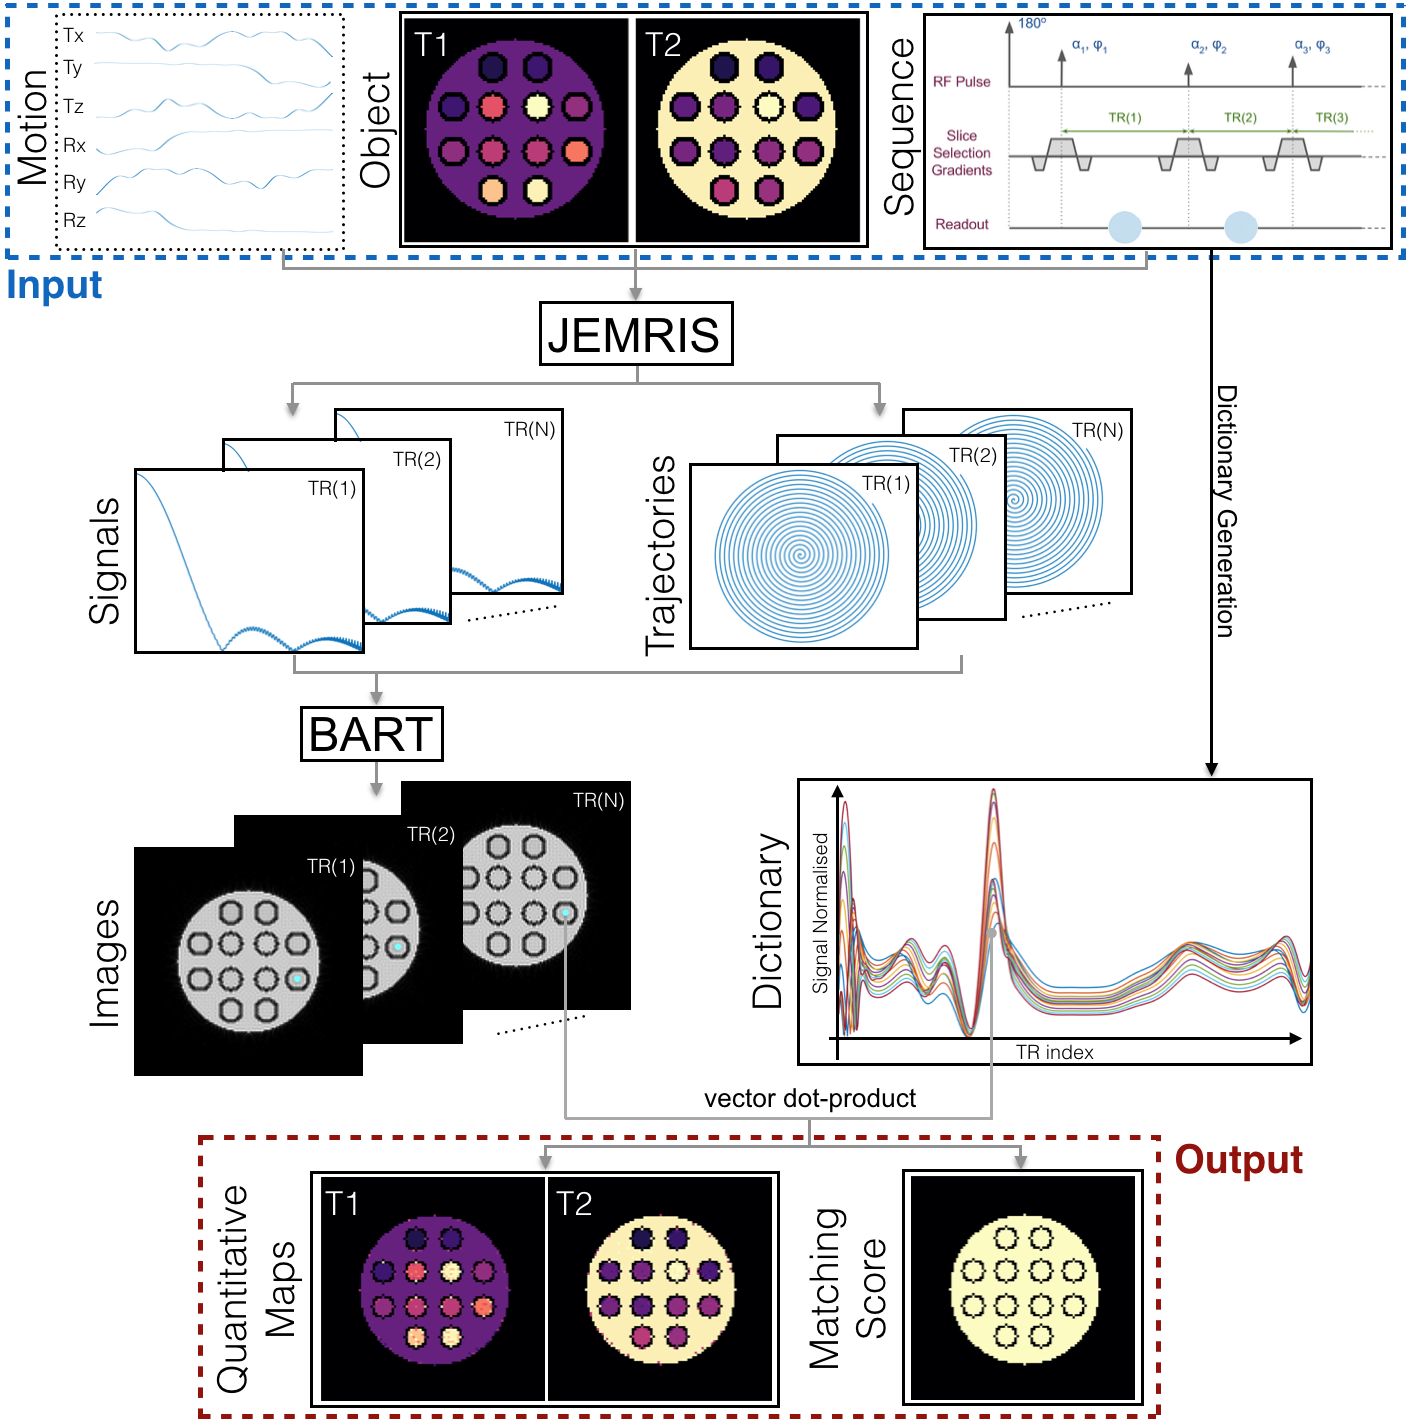
\includegraphics[angle=0,width=1\textwidth, keepaspectratio]{images/mrf/methodFramework}
    \caption{Image space simulation pipeline of a magnetic resonance fingerprinting experiment.
    The framework consists of three inputs: the digital phantom, the MR acquisition sequence and the motion trace. 
    The latter is shown here with dashed lines because it is an optional input parameter. 
    The open source MRI simulator JEMRIS is used to generate signals for each repetition period.
    Then, the BART toolbox is used to reconstruct the images.
    Separately, a dictionary of simulated signals is generated from first principles for a wide range of tissue properties.
    Finally, the quantitative maps are generated together with their corresponding pattern matching scores.}
    \label{fig:methodFramework}
\end{figure}

\hfill

In the following sections we describe every part of our framework in more depth.
We start with the dictionary generation part as this is the first step in an MRF pipeline.
Next, we move on to explaining the image space simulations, together with the motion traces used for the experiments.
Finally, we explain the pattern matching algorithm used to create the quantitative maps.

\hfill

% % % % % % % % % % % % % % % % % % % % % % % % % % % % % % % % % % % % % % % % % % % % % % % % % % % % % % % % % % % % % % % % % % % % % % % % % % % % % % % % % % % % % % % % % % % % % % % % % % % % % % % % % % % % % % % % % % % % % % % % % % % % % % % % % % % % % % % % % % % % % % % % 
\subsection{Dictionary Generation}
\label{method:dictionary}

The first step in an MRF experiment is the creation of a dictionary of simulated signals for a wide variety of tissue properties.
This section presents an overview of the methods used for creating the database of signals for both a bSSFP-type sequence and a FISP-type sequence.

\hfill

\large \textbf{bSSFP Dictionary} \normalsize
The bSSFP dictionary generation is based on the original implementation of the MRF sequence, where Ma et al. \cite{Ma2013} used an inversion-recovery balanced steady state free-precession (bSSFP) sequence (see Figure~\ref{fig:sequencebSSFP}). 
The bSSFP sequence is a type of rapid multi-pulse gradient-echo pulse sequence. 
It is called `rapid' because the repetition time $T_R$ is shorter than both the longitudinal ($T_1$) and the transverse ($T_2$) relaxation times of most known tissue types.
Moreover, it uses balanced (fully rewound) gradients in every direction, thus effectively recovering the transverse magnetisation at the end of each $T_R$ period.

\begin{figure}[ht]
    \centering
    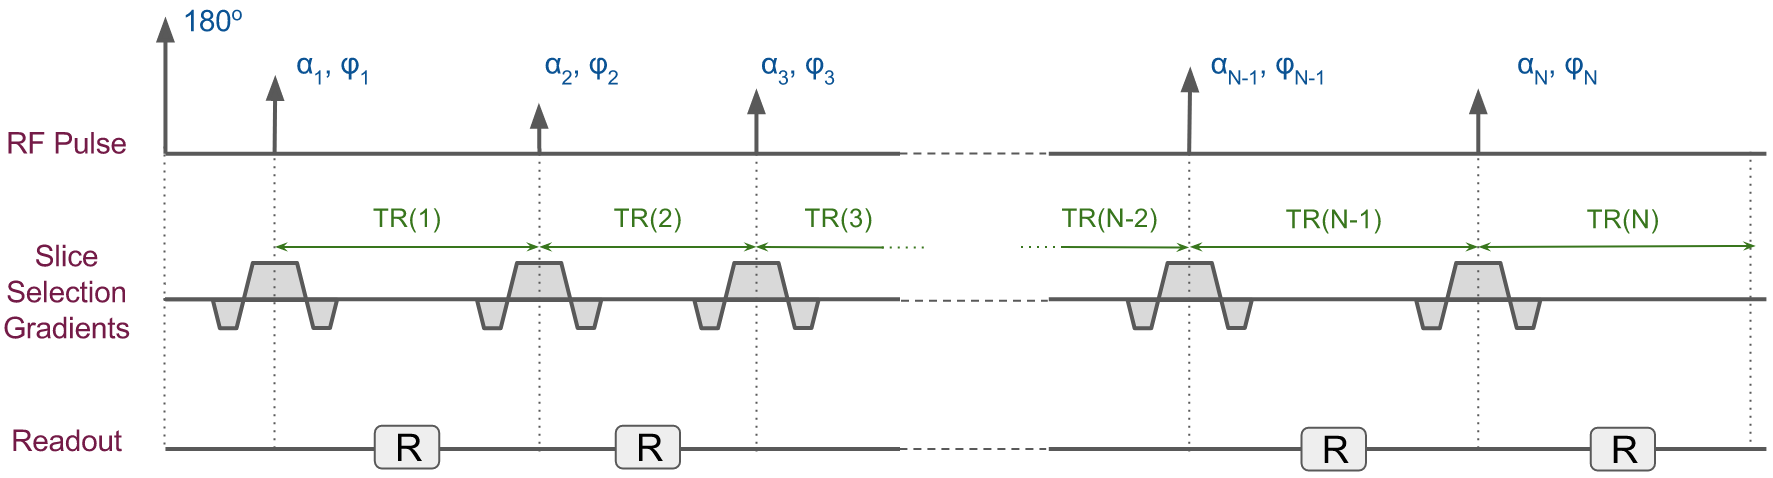
\includegraphics[angle=0,width=1\textwidth, keepaspectratio]{images/mrf/sequencebSSFP}
    \caption{The figure shows a simplified version of an inversion recovery balanced steady state free precession (bSSFP) sequence. 
    All gradients are fully balanced on every direction (they have a net moment of zero at the end of each repetition period) and readout is in the middle of each repetition period.}
    \label{fig:sequencebSSFP}
\end{figure}

\hfill

To model the behaviour of a magnetisation vector with known relaxation times and proton density values in an MRF-bSSFP sequence, we made the following assumptions:

\begin{enumerate}
    \item The object for which we are modelling the magnetisation dynamics in the multi-pulse sequence is considered to be motionless.

    \item The effect of applying an RF pulse of flip angle $\alpha$ and phase angle $\phi$ was considered to be significantly shorter than the relaxation times $T_1$ and $T_2$ and was modelled as happening instantaneously.
    This allowed us to represent its effect as a rotation through the flip angle $\alpha$ about a chosen axis (e.g. the $x$-axis) and a change of coordinate system through the phase angle $\phi$ about the $z$-axis.
    This is detailed in Appendix~\ref{background:rfpulse}.
    
    \item The imaging gradients in this sequence are considered to be fully balanced (all the gradients have zero zeroth moment over each repetition period).
    Thus, any effect induced by the gradients before the readout happens is subsequently reversed by the rewinding gradients.
    We therefore neglected the effect of gradients on the magnetisation vector.

\end{enumerate}

In order to simulate the magnetisation dynamics in this multi-pulse sequence, we first described the effect of a single, arbitrarily chosen, $T_R$ block on a known magnetisation vector (see Figure~\ref{fig:sequencebSSFPOneBlock}).

\hfill

\begin{figure}[ht]
    \centering
    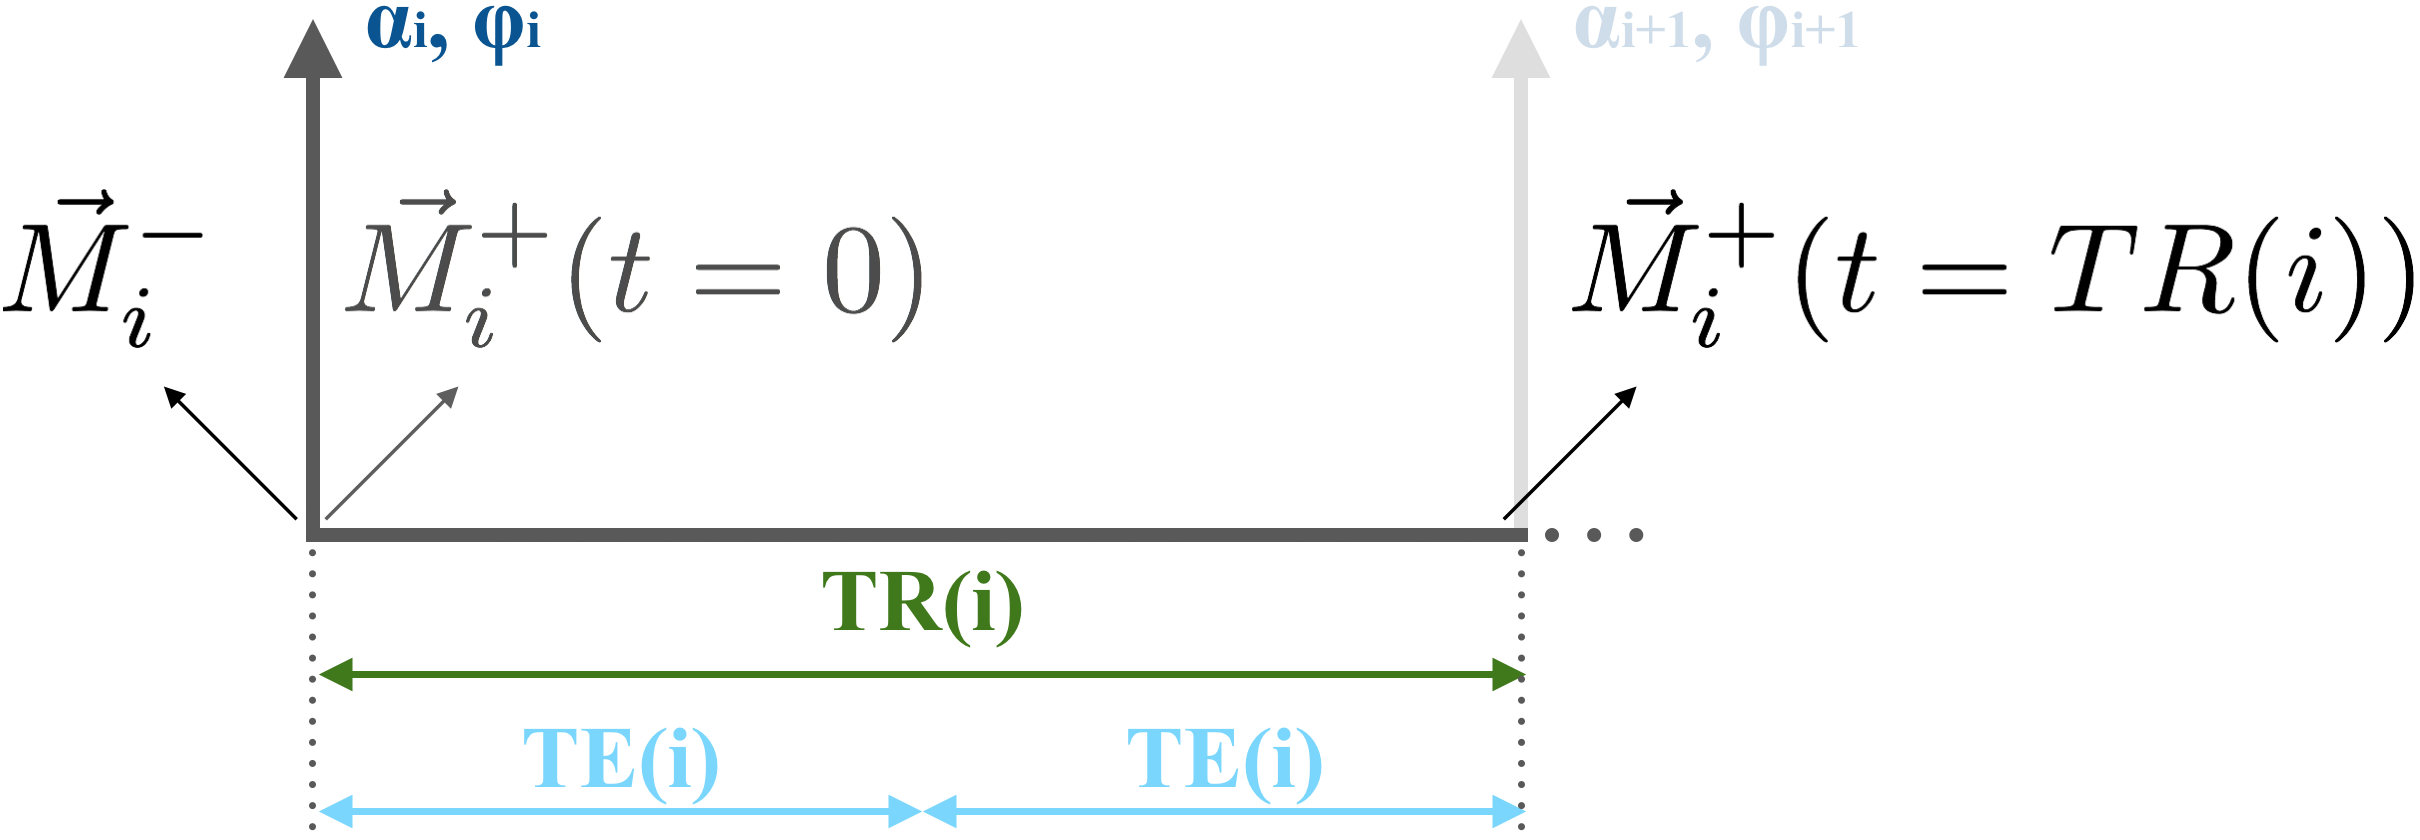
\includegraphics[angle=0,width=0.75\textwidth, keepaspectratio]{images/mrf/sequencebSSFPOneBlock}
    \caption{The figure shows a simplified version of an arbitrarily chosen repetition period block from the bSSFP sequence above.
    The magnetisation vector immediately prior to the $i^{th}$ RF pulse is denoted by $\vec{M}^-_i$ and the magnetisation vector immediately after the $i^{th}$ RF pulse is denoted by $\vec{M}^+_i$.
    The second magnetisation vector is formed as a result of the application of the $i^{th}$ RF pulse with flip angle $\alpha(i)$ on the $\vec{M}^-_i$ vector.
    Similarly, $\vec{M}^-_{i+1}$ and $\vec{M}^+_{i+1}$ are the magnetisation vectors immediately before and after the $(i+1)^{th}$ RF pulse.
    Moreover, the relationship between $\vec{M}^+_{i}$ and $\vec{M}^-_{i+1}$ is given by: $ \vec{M}^-_{i+1} = \vec{M}^+_{i}(t = TR(i))$, where $t \in [0, TR(i)]$ }
    \label{fig:sequencebSSFPOneBlock}
\end{figure}

Let us first define the magnetisation vector immediately prior to the $i^{th}$ RF pulse:
\begin{equation}
    M^{-}_i \equiv \big[ M^-_{x_i} \, \,  M^-_{y_i} \, \, M^-_{z_i} \big]^T
\end{equation}
and immediately after the $i^{th}$ RF pulse:
\begin{equation}
    M^{+}_i \equiv \big[ M^+_{x_i} \, \,  M^+_{y_i} \, \, M^+_{z_i} \big]^T
\end{equation}
\textbf{RF Pulse event.} The effect of an instantaneous RF pulse with flip angle $\alpha_i$ and phase angle $\phi_i$ links the two vectors through rotation matrices:
\begin{equation}
    \begin{split}
        M^{+}_i & = R_{z}(-\phi_i) R_{x}(-\alpha_i) R_{z}(\phi_i) M^{-}_i  \\
        \text{where:}         & \\
        & R_x(\alpha) = 
            \begin{bmatrix}
                1 &       0     &       0      \\
                0 & \cos(\alpha) & -\sin(\alpha) \\
                0 & \sin(\alpha) & \phantom{-}\cos(\alpha)
            \end{bmatrix} \\
        & R_z(\phi) = 
            \begin{bmatrix}
    	        \cos(\phi) & -\sin(\phi) & 0 \\
                \sin(\phi) & \phantom{-}\cos(\phi) & 0 \\
                    0   &      0     & 1
            \end{bmatrix}
    \end{split}
\end{equation}

\textbf{Relaxation event.} Next, as the effect induced by the gradients can be neglected, the magnetisation vector will begin the process of returning to its equilibrium state.
This phenomenon is governed by the $T_1$ and $T_2$ relaxation times of the tissue being modelled and can be described using matrix notation.
To fully describe the process there are two matrices involved; the diagonal matrix $D$:

\begin{equation}
    D ( t ) = \left[
    \begin{array}{c c c}
          E_2(t) &     0      &     0 \\
           0      & E_2(t) &     0 \\
           0      &     0      & E_1(t)
    \end{array}
    \right]
\end{equation}

and the column matrix $C$:
\begin{equation}
    C ( t ) = \left[
    \begin{array}{c}
        0 \\
        0 \\
    M_0(1 - E_1(t))
    \end{array}
    \right]
\end{equation}
where $E_1(t) \equiv e^{-t/T_1}$ and $E_2(t) \equiv e^{-t/T_2}$.
These equations have been previously defined in Section~\ref{chapterlabel2sec1Bloch}.
In the rotating reference frame (after demodulating with the Larmor frequency $\omega_0$), this process can therefore be described as:
\begin{equation}
    M^{+}_i (t)  = D(t) M^{+}_i (0) + C(t)
\end{equation}
By choosing $t = T_{E_i}$ or $t = T_{R_i}$, we can calculate the magnetisation vector components at readout time $T_E$ after the $i^{th}$ RF pulse, or at the end of the $i^{th}$ repetition period.

\hfill

\textbf{Off-resonance event.} However, if there are any spatially invariant static field inhomogeneities $\Delta B$ present, the phase of the magnetisation vector will change over a given repetition time period. 
This phase will be determined by $\beta(t) = \gamma \Delta B t = \Delta \omega t = 2\pi \Delta \nu t$ during any $T_R$ block.
To model the behaviour of phase accrual, we use a rotation about the $z$ axis of the magnetisation vector.
This can be mathematically represented as:
\begin{equation}
    M^{+}_i (t)  = R_z(\beta(t)) M^{+}_i (0)
\end{equation}
where the rotation matrix $R_z$ has been previously described and $\beta(t) = 2\pi \, \, \Delta \nu \, \, t$ is the accumulated phase due to off-resonance frequency $\Delta \nu$ at time $t$ during the $i^{th}$ repetition period. 
Again, we can choose $t = T_{E_i}$ or $t = T_{R_i}$ to calculate the magnetisation vector components at the echo time or at the end of a repetition period, respectively.

\hfill

\textbf{Linking the events.} These three events, RF pulse, relaxation and off-resonance effects, fully describe the magnetisation dynamics of a spin ensemble with equilibrium magnetisation $M_0$, relaxation constants $T_1$ and $T_2$, and with off-resonance frequency $\Delta \nu$.
These events can now be linked together to calculate the magnetisation vector at time $t$ after the $i^{th}$ RF pulse:
\begin{equation}
    M^{+}_i (t) = D(t) R_z(\beta(t)) \big( R_{z}(\phi_i) R_{x}(-\alpha_i) R_{z}(-\phi_i) M^{-}_i \big) + C(t)
\end{equation}

\textbf{Dictionary.} However, the dictionary is made up of signals generated for a wide range of tissue properties.
More specifically, every signal can be labeled with a `tissue tuple':
$(T_{1_j}, T_{2_j}, \Delta f_{j})$, with $j \in [1, M]$, where $M$ is the total number of tuples.
Therefore, to create the dictionary, the process needs to be repeated for each tissue type.

\hfill

The dictionary was created in MATLAB using a vectorised version of the previously described process.
The speed of our method comes from the fact that we calculate the magnetisation vector components of all tissue types simultaneously, for every $T_R$ period.
For this, we start by defining a $3 \times M$ matrix for the $M_x, \, M_y, \, M_z$ components of the magnetisation vector for all $M$ tissue types immediately before the $i^{th}$ RF Pulse:
\begin{equation}
    M^{-}_i = 
    \begin{bmatrix}
        M_{ix_1} & M_{ix_2} & \dots & M_{ix_M} \\
        M_{iy_1} & M_{iy_2} & \dots & M_{iy_M} \\
        M_{iz_1} & M_{iz_2} & \dots & M_{iz_M}
    \end{bmatrix}
\end{equation}

To flip the magnetisation vector for all the tissue types, we precompute the RF pulse matrix for the current repetition period:
\begin{equation}
        R_{RF_i} = R_{z}(\phi_i) R_{x}(-\alpha_i) R_{z}(-\phi_i)
\end{equation}
and then apply this to our previously defined $3 \times M$ matrix of magnetisation vector components:
\begin{equation}
    M^{+}_i(0) = R_{RF_i} \, \, M^{-}_i
\end{equation}

For the off-resonance effects, we split the process in two.
We create two $3 \times M$ matrices to represent the effect of rotation about the z-axis for all possible $\beta_j(t) = 2\pi \Delta \nu_j \, t$ \big(with $j \in [1, M]$ \big) off-resonance angles.
Mathematically, this is given by:
\begin{equation}
    M^{+}_i (t) = R_{\Delta \nu_1}(t) \, \odot \, M^{+}_i(0) + R_{\Delta \nu_2}(t)  \, \odot \, M^{+}_i(0)^{(p)}
\end{equation}

where $\odot$ denotes component-wise multiplication, and:

\begin{equation}
    R_{\Delta \nu_1}(t)  = \begin{bmatrix} \phantom{-}\cos(\beta_{1}(t) ) & \phantom{-}\cos(\beta_{2}(t) ) & \dots & \phantom{-}\cos(\beta_{M}(t) ) \\
    \phantom{-}\cos(\beta_{1}(t) ) & \phantom{-}\cos(\beta_{2}(t) ) & \dots & \phantom{-}\cos(\beta_{M}(t) ) \\
    1    &        1   & \dots &  1
    \end{bmatrix}
\end{equation}

\begin{equation}
    R_{\Delta \nu_2}(t)  = \begin{bmatrix} -\sin(\beta_{1}(t) ) & -\sin(\beta_{2}(t) ) & \dots & -\sin(\beta_{M}(t) ) \\
    \phantom{-}\sin(\beta_{1}(t) ) & \phantom{-}\sin(\beta_{2}(t) ) & \dots & \phantom{-}\sin(\beta_{M}(t) ) \\
    0     &      0      & \dots &      0
    \end{bmatrix}
\end{equation}

\begin{equation}
\begin{split}
    M^{+}_i(0) = &
    \begin{bmatrix}
        M^{+}_{ix_1}(0) & M^{+}_{ix_2}(0) & \dots & M^{+}_{ix_M}(0) \\
        M^{+}_{iy_1}(0) & M^{+}_{iy_2}(0) & \dots & M^{+}_{iy_M}(0) \\
        M^{+}_{iz_1}(0) & M^{+}_{iz_2}(0) & \dots & M^{+}_{iz_M}(0)
    \end{bmatrix} \\
    = & \, \, R_{RF_i} \, \, M^{-}_i \text{ (as previously defined)}
\end{split}
\end{equation}

\begin{equation}
\begin{split}
    M^{+}_i(0)^{(p)} = &
    \begin{bmatrix}
        M^{+}_{iy_1}(0) & M^{+}_{iy_2}(0) & \dots & M^{+}_{iy_M}(0) \\
        M^{+}_{ix_1}(0) & M^{+}_{ix_2}(0) & \dots & M^{+}_{ix_M}(0) \\
        M^{+}_{iz_1}(0) & M^{+}_{iz_2}(0) & \dots & M^{+}_{iz_M}(0)
    \end{bmatrix} \\
    & \text{ (Obs: lines 1 and 2 have been permuted)}
\end{split}
\end{equation}

For the relaxation effects, we again build two $3 \times M$ matrices to account for all M combinations of $T_1$ and $T_2$ decay rates:
\begin{equation}
    M^{+}_i(t) = D(t)  \, \odot \, M^{+}_i(0) + C(t) 
\end{equation}

where, again, $\odot$ denotes component-wise multiplication, and:

\begin{equation}
    D(t)  = 
    \begin{bmatrix}
        E_{2_1}(t)  & E_{2_2}(t)  & \dots & E_{2_M}(t)  \\
        E_{2_1}(t)  & E_{2_2}(t)  & \dots & E_{2_M}(t)  \\
        E_{1_1}(t)  & E_{1_2}(t)  & \dots & E_{1_M}(t)  
    \end{bmatrix}
\end{equation}

and

\begin{equation}
    C(t)  = 
    \begin{bmatrix}
        0 & 0 & \dots & 0 \\
        0 & 0 & \dots & 0 \\
        1 - E_{1_1}(t)  & 1- E_{1_2}(t)  & \dots & 1- E_{1_M}(t)  
    \end{bmatrix} 
\end{equation}

where $E_{1_j}(t) \equiv e^{-t/T_{1_j}}$ and $E_{2_j}(t) \equiv e^{-t/T_{2_j}}$, with $j \in [1, M]$.

\hfill 

This process is then repeated, in order, for all repetition times in the sequence.
At the end, a dictionary of M signals, each with N time points is constructed.
For completion, we store all 3 components of the magnetic moment vectors, thus having an $M \times N \times 3$ dictionary matrix.
Pseudocode for the created algorithms can be found in Appendix~\ref{appendixlabel1}.

\hfill

\large \textbf{FISP Dictionary} \normalsize
More recently, Jiang et al. \cite{Jiang2015} used an inversion-recovery fast imaging with steady state precession (FISP) sequence (see Figure~\ref{fig:sequenceFISP}). 
Similar to bSSFP, FISP is also a type of rapid multi-pulse gradient-echo sequence which uses short repetition times.
In contrast to the previous sequence, FISP uses an unbalanced gradient in one or multiple gradient directions, thus `spoiling' the transverse magnetization prior to the next RF pulse. 
Gradient spoiling does not effectively null the transverse magnetization, so then both the longitudinal and the transverse magnetization will contribute to the signal in the next cycle.

\begin{figure}[ht]
    \centering
    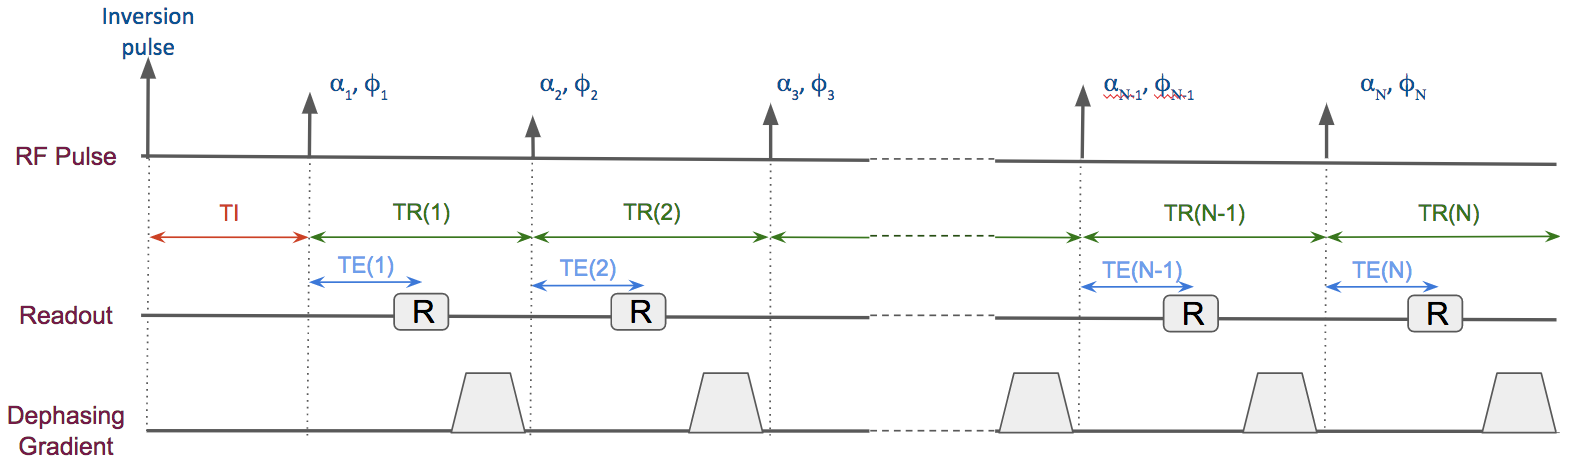
\includegraphics[angle=0,width=1\textwidth, keepaspectratio]{images/mrf/sequenceFISP}
    \caption{Simplified version of a fast imaging with steady state precession (FISP) sequence. It contains an unbalanced `spoiler' gradient in each each repetition period.}
    \label{fig:sequenceFISP}
\end{figure}

\hfill

FISP-type sequences are used in Magnetic Resonance Fingerprinting due to their fast imaging characteristics and their immunity to banding artefacts commonly seen in fully balanced steady state sequences. 
These banding artefacts are present due to inhomogeneities in the main magnetic field caused by susceptibility variations or poor magnet shimming. 

\hfill

In terms of simulating the behaviour of a magnetisation vector with known relaxation times and proton density values in an MRF-FISP sequence, single isochromat Bloch equations are no longer feasible.
Due to the presence of a strong dephasing gradient and repetition times shorter than the transverse relaxations of most tissue types \big($T_R \leq T_2$\big), the transverse magnetisation will not be destroyed, but completely dephased across a voxel.
To model this, Bloch equations can be used, but a large number of isochromats needs to be simulated to achieve accuracy.
For this, a different approach was used, called the Extended Phase Graph formalism \cite{Hennig1988} \cite{Hennig1991}.

\hfill

\textbf{Extended Phase Graph Formalism.} The EPG algorithm \cite{Hennig1988} \cite{Hennig1991} \cite{Weigel2015} is a tool used to simulate signals obtained from a wide variety of MRI pulse sequences.
Similar to the Bloch equations approach, EPG characterizes a given sequence through the effects of RF pulses, relaxation constants, and dephasing due to gradients or inhomogeneities in the main magnetic field.
However, unlike the classic Bloch equations approach, EPG describes a spin system as a discrete set of phase states (or, `configuration states') \cite{Hennig1988}.

\hfill

To understand how EPG works, we will first define the total magnetisation $M$ at thermal equilibrium as a normalised column vector $B = [0 \, 0 \, 1]^T$.
$B$ contains the coefficients for the $M_x$, $M_y$ and $M_z$ components of the total magnetisation M.
At any time point during a multi-pulse experiment, one can calculate the total magnetisation by summing over a collection of spins which are described by their corresponding x,y,z components.
However, to be accurate, this requires a large spin ensemble.

\hfill

\textbf{Substates.} In the EPG formalism the matrix $B$ is expanded to describe \textit{substates}.
These substates are defined as collection of spins with different $M_x$, $M_y$ and $M_z$ components and are characterised by the net magnetisation of the substate, and the space-dependent phase of the transverse magnetisation of the spin ensemble \cite{Hennig1988}.
In this framework, the signal intensity at any given time point during the sequence can be calculated by knowing the partitioning of the total magnetisation between the substates, and the net magnetisation in each substate.

\hfill

For a single-voxel multi-pulse FISP experiment let us now consider that the gradient's moment induces the same amount of dephasing across this voxel during a fixed time period $\Delta t$ at the end of each repetition period.
For an idealised gradient and an idealised voxel with uniform density of magnetisation,
the amount of dephasing is defined by the interval $[-\pi, \pi]$.

\hfill 

Let us consider that the first RF pulse is an ideal $90^o$ excitation pulse which flips the total magnetisation in the transverse plane.
Prior to the second RF pulse, due to the presence of the idealised dephasing gradient,
the spins will accrue different phases, ranging from $-\pi$ in one corner of the voxel, to $+\pi$ in the opposite corner.
This state in which the transverse magnetisation is now found is called $F_1$ \cite{Hennig1988} \cite{Scheffler1999} and can be conceptually described as an evenly distributed collection of magnetisation vectors over the transverse plane (see Figure~\ref{fig:F1state}). 

\begin{figure}[ht]
    \centering
    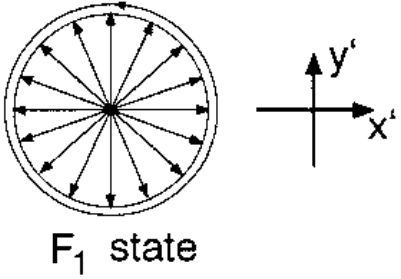
\includegraphics[angle=0,width=0.4\textwidth, keepaspectratio]{images/mrf/F1state}
    \caption{The $F_1$ state is a magnetisation substate which describes a uniform distribution of magnetisation vectors over the transverse plane, with phases ranging from $-\pi$ to $+\pi$. Figure adapted from \cite{Scheffler1999}.}
    \label{fig:F1state}
\end{figure}

\hfill

The application of a second RF pulse will interfere with this state.
For an arbitrary flip angle $\alpha$ and phase angle $\phi = 0$, the $F_1$ `disk' will be rotated around the RF pulse's axis of rotation.
The newly formed transverse magnetisation can be described as two dephased states: $F^+_1$ and $F^+_{-1}$, while the longitudinal magnetisation is now known as $Z^+_1$.
The superscript `+' denotes `immediately after the RF pulse'.
In the EPG formalism, other states exist and they are denoted as $F_n$, depending on the amount of dephasing experienced.
This can be seen in Figure~\ref{fig:EPGeffectofgrad}, where the $2^{nd}$ gradient pulse further dephased the $F_1$ state.
Due to being an idealised gradient and an idealised voxel with uniform density of magnetisation, the amount of dephasing is again defined by the interval $[-\pi, \pi]$.
This causes the spins to have now accrued phases ranging from $-2 \pi$ to $+2 \pi$.
The presence of the gradient will therefore `transform' the $F_1^+$ state into a new state we call $F_2$.
On the other hand, $Z^+_1$ was formed because the RF pulse `flipped' the transverse components of some of the pre-RF pulse magnetisation vectors into the longitudinal plane.
The formation of the $F_1^+$, $F_{-1}^+$ and $Z_1^+$ states is better understood through the Woessner decomposition \cite{Woessner1961}.

\begin{figure}[ht]
    \centering
    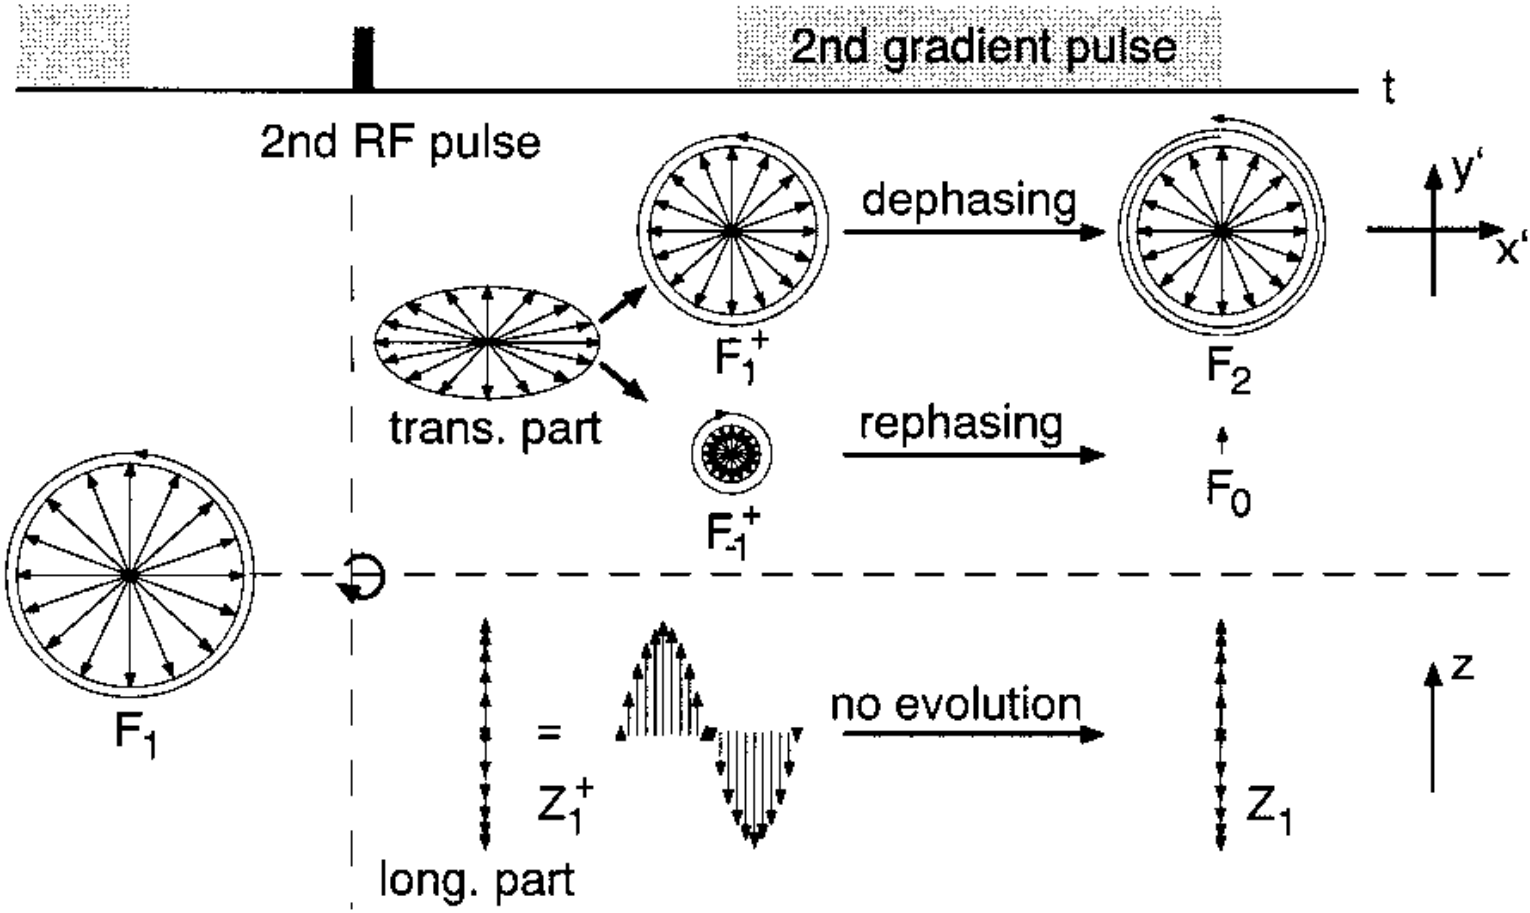
\includegraphics[angle=0,width=0.8\textwidth, keepaspectratio]{images/mrf/EPGeffectofgrad}
    \caption{A second RF pulse will `split' the previous $F_1$ configuration into two separate transverse state configurations $F_1^+$ and $F_{-1}^+$, and a longitudinal state $Z_1^+$; this process is best described with the \textit{Woessner decomposition}. During the application of the dephasing gradient, the longitudinal state remains unaffected, while the transverse states are further dephased $F_1^+ \rightarrow F_2$, and rephased $F_{-1}^+ \rightarrow F_0$, respectively. Figure adapted from \cite{Scheffler1999}.}
    \label{fig:EPGeffectofgrad}
\end{figure}

\hfill

\textbf{Woessner decomposition.} The Woessner decomposition describes the behaviour of a complex magnetisation vector $F = M_x + i M_y$ subject to an RF pulse of arbitrary flip angle $\alpha$ and phase angle $\phi$.
As stated before, the effect of an RF pulse can be written as a rotation matrix, which, when applied to the complex magnetisation vector yields \cite{Haacke1999} \cite{Scheffler1999}:

\begin{equation}\label{eq:woessner}
\begin{split}
    F^+ &= F^- cos^2(\alpha/2) + e^{2i\phi} (F^-)^* sin^2(\alpha/2)  - i e^{i \phi} M_z^- sin(\alpha)  \\
    M_z^+ &= - i/2 e^{-i \phi} F^- sin(\alpha) + i/2 e^{-i \phi} (F^-)^* sin(\alpha) + M_z^- cos(\alpha) 
\end{split}
\end{equation}
where the superscript \textbf{+} represents immediately `after the RF pulse' and the superscript \textbf{-} represents immediately `before the RF pulse'.

\hfill

To make the transition to fully dephased transverse states $F_n$ and longitudinal states $Z_n$, we need to take into account the fact that an $F_n$ state represents a collection of dephased spins at different spatial positions within the idealised voxel.
For a one-dimensional voxel, the phase of a spin at position $x$ induced by n identical gradient lobes evolves with $e^{i \, n \, \, \gamma G_x x \, \Delta t }$, where $G_x$ is the amplitude of the gradient and $\Delta t$ is its duration.
For all positions r in the voxel, the dephased transversal state can be written as a sum over all positions: $ F_n \int_r \, dr \, e^{i \, n \, \, \gamma G r \, \Delta t }$, where the amplitude of the complex number $F_n$ represents the magnitude of this state's population.
Similarly, the longitudinal state can be described as $ Z_n \int_r \, dr \, e^{i \, n \, \, \gamma G r \, \Delta t }$.

\hfill

\textbf{RF Pulse. } Introducing the complex dephased states in equations \ref{eq:woessner} and transforming into matrix representation, we can write:

\begin{equation}\label{eq:woessnerFn1}
    \begin{bmatrix}
        F_n      \\
        F_{-n}^* \\
        Z_n
    \end{bmatrix}^+ = 
    T_{\phi}(\alpha)
    \begin{bmatrix}
        F_n      \\
        F_{-n}^* \\
        Z_n
    \end{bmatrix}^- 
\end{equation}
where
\begin{equation}\label{eq:woessnerFn2}
    T_{\phi}(\alpha) = 
    \begin{bmatrix}
        cos^2(\alpha/2) & e^{2i\phi} sin^2(\alpha/2) & - i e^{i \phi} sin(\alpha) \\
        e^{-2i\phi} sin^2(\alpha/2) & cos^2(\alpha/2) & i e^{-i \phi} sin(\alpha) \\
        - i/2 e^{-i \phi} sin(\alpha) & i/2 e^{i \phi} sin(\alpha) & cos \alpha
    \end{bmatrix}
\end{equation}

and the $F^*_{-n}$ state represents the complex conjugate of the $F_n$ state.

\hfill

Equations \ref{eq:woessnerFn1} and \ref{eq:woessnerFn2} show that, given an ensemble of spins, an RF pulse with flip angle $\alpha$ and phase angle $\phi$ will redistribute the population into different states.
For example, different amounts of the pre-RF pulse $F^-_n$ state can now be found in both the post-RF pulse transverse state $F^+_n$ and the longitudinal state $Z_n$.
The population represented by $F^*_{-n}$ state can be interpreted as an isochromat population whose phase was instantaneously inverted by the RF pulse, and which can be rephased later.

\hfill

\textbf{Dephasing. } In this framework, the dephasing induced by an idealised gradient can be described simply as a transition between two adjacent states.
More specifically, the application of the $(n+1)^{th}$ gradient lobe of equal size and timing as the previous ones will shift the transverse states from $F_n$ to $F_{n+1}$.
An example is shown in Figure~\ref{fig:EPGeffectofgrad}.

\hfill

\textbf{Relaxation Effects. } The effects of relaxation towards thermal equilibrium can also be described in this framework.
For the transverse states $T_2$ relaxation occurs: $F_n = E_2 F_n^+$, while for the longitudinal states $T_1$ relaxation occurs: $Z_n = E_1 Z_n^+$, for $n \neq 0$ and $Z_0 = E_1 Z_0^+ + M_0(1 - E_1)$ where $E_1 = e^{-\tau/T_1}$, $E_2 = e^{-\tau/T_2}$ for a given time $\tau$.
In matrix form, this becomes:

\begin{equation}\label{eq:woessnerFn}
    \begin{bmatrix}
        F_n      \\
        F_{-n}^* \\
        Z_n
    \end{bmatrix}^+ = 
    \underbrace{
    \underbrace{\begin{bmatrix}
        E_2 & 0 & 0 \\
        0 & E_2 & 0 \\
        0 & 0 & E_1 
    \end{bmatrix}
    \begin{bmatrix}
        F_n      \\
        F_{-n}^* \\
        Z_n
    \end{bmatrix}^-}_\text{for n $\neq$ 0}
    +
    \begin{bmatrix}
        0 \\
        0 \\
        M_0 (1 - E_1)
    \end{bmatrix}}_\text{for n = 0}
\end{equation}

\hfill

\textbf{The Extended Phase Graph algorithm. } In the EPG algorithm the set of all possible confugration states at any given time point is stored in a matrix called `state matrix':
\begin{equation}
    \Omega = 
    \begin{bmatrix}
    \widetilde{F}_0 & \widetilde{F}_1 & \widetilde{F}_2 & \dots \\
    \widetilde{F}_0^* & \widetilde{F}_{-1}^* & \widetilde{F}_{-2}^* & \dots \\
    \widetilde{Z}_0 & \widetilde{Z}_1 & \widetilde{Z}_2 & \dots 
    \end{bmatrix}
\end{equation}

To store all the possible configuration states for all time points $t$ in the multi-pulse sequence, the following `evolution matrices' are used:

\begin{equation}
    \Xi_F = 
    \begin{bmatrix}
    \vdots & \vdots & \vdots & \vdots & \dots \\
    \widetilde{F}_2(t_0) & \widetilde{F}_2(t_1) & \widetilde{F}_2(t_2) & \widetilde{F}_2(t_3) & \dots \\
    \widetilde{F}_1(t_0) & \widetilde{F}_1(t_1) & \widetilde{F}_1(t_2) & \widetilde{F}_1(t_3) & \dots \\
    \widetilde{F}_0(t_0) & \widetilde{F}_0(t_1) & \widetilde{F}_0(t_2) & \widetilde{F}_0(t_3) & \dots \\
    \widetilde{F}^*_{-1}(t_0) & \widetilde{F}^*_{-1}(t_1) & \widetilde{F}^*_{-1}(t_2) & \widetilde{F}^*_{-1}(t_3) & \dots \\
    \widetilde{F}^*_{-2}(t_0) & \widetilde{F}^*_{-2}(t_1) & \widetilde{F}^*_{-2}(t_2) & \widetilde{F}^*_{-2}(t_3) & \dots \\
    \vdots & \vdots & \vdots & \vdots & \dots 
    \end{bmatrix}
\end{equation}

and

\begin{equation}
    \Xi_Z = 
    \begin{bmatrix}
    \vdots & \vdots & \vdots & \vdots & \dots \\
    \widetilde{Z}_2(t_0) & \widetilde{Z}_2(t_1) & \widetilde{Z}_2(t_2) & \widetilde{Z}_2(t_3) & \dots \\
    \widetilde{Z}_1(t_0) & \widetilde{Z}_1(t_1) & \widetilde{Z}_1(t_2) & \widetilde{Z}_1(t_3) & \dots \\
    \widetilde{Z}_0(t_0) & \widetilde{Z}_0(t_1) & \widetilde{Z}_0(t_2) & \widetilde{Z}_0(t_3) & \dots 
    \end{bmatrix}
\end{equation}

\hfill

To describe the evolution of the system through a multi-pulse sequence, we start with $\Omega (t < 0) = [0, 0, 1]^T$, and then sequentially apply the operators corresponding to an event.
For example, if the first event is an RF pulse of flip angle $\alpha = 90^o$ and phase angle $\phi = 0^o$, we write:
\begin{equation}
    \Omega (t = 0) = T_x(90^o) \Omega (t < 0) = 
    \begin{bmatrix} 
        F_0 \\
        F^*_0 \\
        Z_0
    \end{bmatrix} = 
    \begin{bmatrix} 
        0 \\
        0 \\
        1
    \end{bmatrix}
\end{equation}

Then, if the next event is constant dephasing until the end of the $T_R$ block, we calculate the state matrix as:
\begin{equation}
    \Omega (t = T_R) = S \, \, T_x(90^o) \Omega (t < 0) = 
    \begin{bmatrix} 
        0 & 1\\
        0 & 0\\
        0 & 0
    \end{bmatrix}
\end{equation}
where $S$ is the shift operator which performs $F_n \rightarrow F_{n+1}$ and leaves the longitudinal state unchanged $Z_n \rightarrow Z_n$. 
Note that the state matrix contains all possible states, which means that for our example $F_{-1}^* = 0$ was shifted to $F_0^*$.

\hfill

\textbf{Dictionary.} To create the MRF-FISP dictionary, the EPG algorithm was used.
As with the bSSFP case, a signal of N time points is created for each `tissue tuple'
$(T_{1_j}, T_{2_j})$, with $j \in [1, M]$, where $M$ is the total number of tuples.
For the FISP dictionary, off-resonance frequencies were not included.
The sequence used is found in Figure~\ref{fig:sequenceFISP}, where the echo times were kept constant for every repetition block, and the unbalanced gradients achieved the same amount of dephasing in each $T_R$.

\hfill

To generate the signal for a given tissue type, the process described above was used.
Starting from thermal equilibrium, the effect of the sequence was represented as three types of events applied sequentially.
More specifically, as the number of RF pulses is known \textit{a priori} to be equal to $N$, two state matrices were constructed: $\Omega^{-RF}$ - a $(3 \times (N+1))$ matrix representing the transverse and longitudinal states immediately before each RF pulse, and $\Omega^{+RF}$ - a $(3 \times N)$ matrix representing the transverse and longitudinal states immediately after each RF pulse.
Then, for every $i^{th}$ $T_R$ block the pre-$(i+1)^{th}$ RF pulse state matrix was calculated by chaining the RF Pulse, relaxation and dephasing events.

\hfill

The dictionary was created in MATLAB using the process described above.
For every tissue type, the signal was calculated as the $F_0$ state at each readout time point in the sequence.
As all the other states are completely dephased, it follows that only the $F_0$ states contribute to the signal.
The dictionary is then stored as an $M \times N$ matrix of complex values.
Pseudocode for the algorithm can be found in Appendix~\ref{appendixlabel2}.

\hfill

% % % % % % % % % % % % % % % % % % % % % % % % % % % % % % % % % % % % % % % % % % % % % % % % % % % % % % % % % % % % % % % % % % % % % % % % % % % % % % % % % % % % % % % % % % % % % % % % % % % % % % % % % % % % % % % % % % % % % % % % % % % % % % % % % % % % % % % % % % % % % % % % 
\subsection{Image Space Simulation}
\label{method:imagespace}

% % % % % % % % % % % % 
\subsubsection{Digital Object}

For the simulations involved we created a digital phantom of $80mm$ in diameter, consisting of 12 circular structures of $5mm$ in diameter.
The resolution of this phantom is of $1mm$, and the spin density was chosen such that there is a single spin isochromat present at each spatial location $\vec{r}$ in the phantom.
The distribution of $T_1$ and $T_2$ relaxation times is shown in Figure~\ref{fig:inputObject}, while the spin density is set to $\rho(\vec{r}) = 1$ everywhere inside the phantom, except for the space between the `tubes' and the circular phantom.
The range of values chosen for the relaxation times are also summarised in Appendix~\ref{appendixlabelPhantom}.

\begin{figure}[ht]
    \centering
    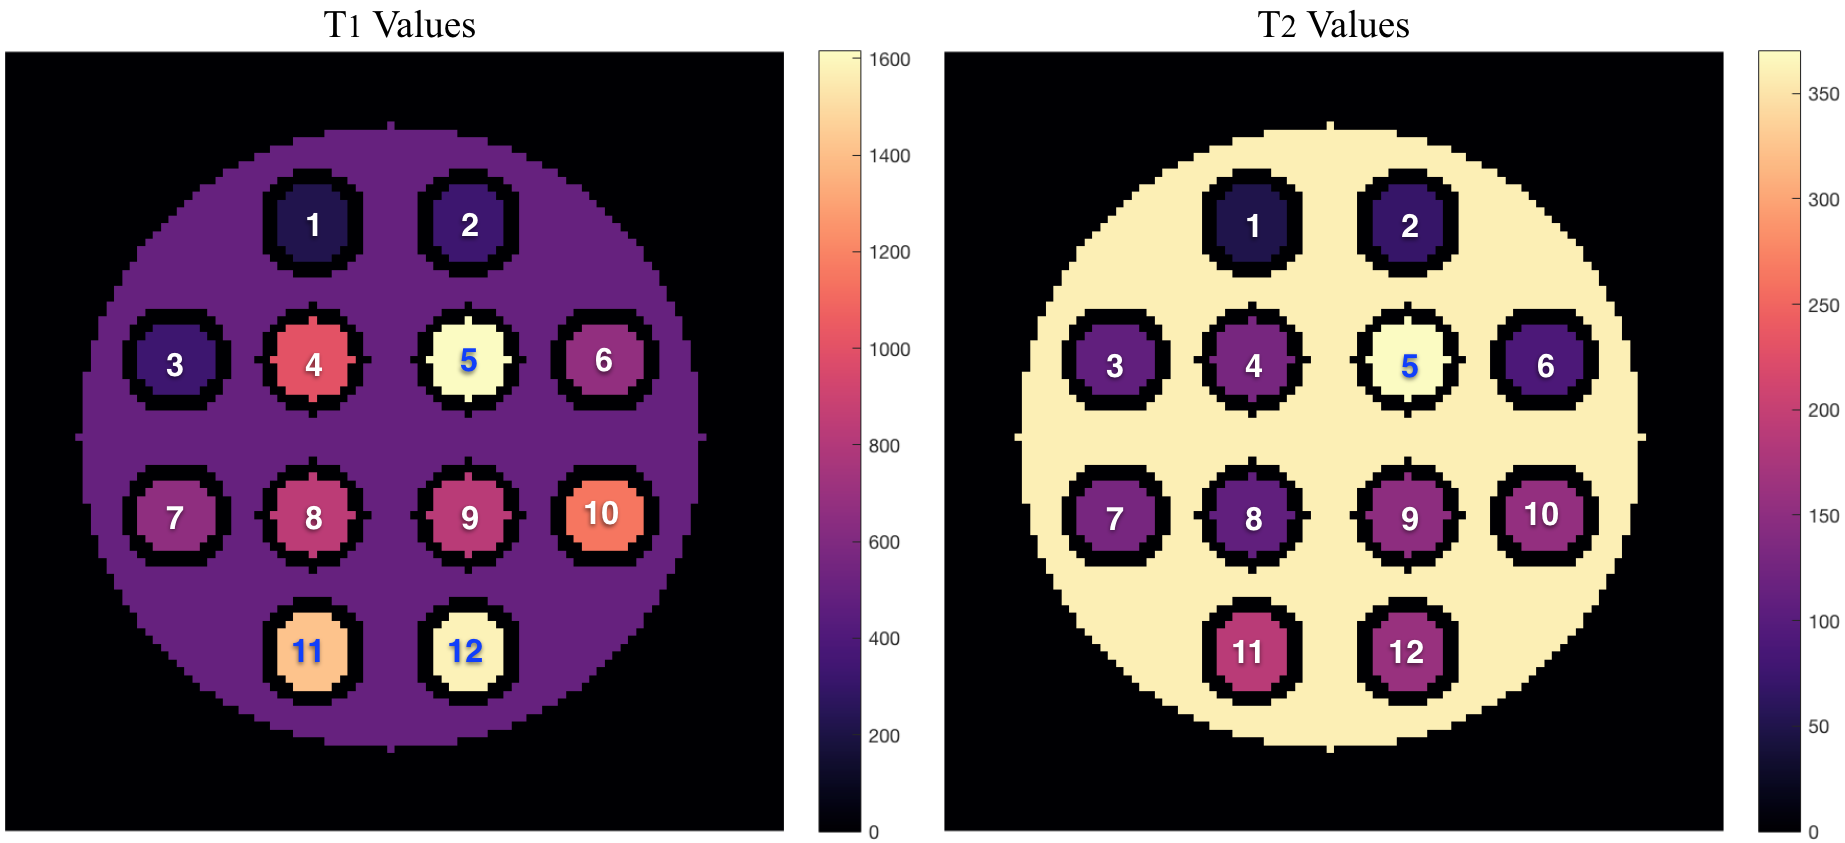
\includegraphics[angle=0,width=1\textwidth, keepaspectratio]{images/mrf/inputObject}
    \caption{The input object is a circular phantom of $80mm$ in diameter, consisting of 12 circular structures of $5mm$ in diameter. Each `tube' (shown here with indices ranging from 1 to 12) has a different $T_1$ and $T_2$ value. Similarly, the surrounding structure has its own relaxation parameters (index 0). $T_1$ and $T_2$ values are summarised in a table in Appendix~\ref{appendixlabelPhantom}.}
    \label{fig:inputObject}
\end{figure}

\hfill

The choice of digital phantom structure and composition is based on the \textit{Eurospin} 
phantom set, Test Object 5 (TO5), which contains 12 holes for agarose gel sample tubes with different relaxation properties \cite{Ihalainen2004} (see Figure~\ref{fig:realPhantom}).
The values for the relaxation times were chosen from the provided $T_1$ and $T_2$ Eurospin Appendix table and correspond to 12 of the 18 available tubes.
Moreover, this type of phantom was used in previous MRF studies such as those presented in \cite{Doneva2016} and \cite{Sommer2017}.

\begin{figure}[ht]
    \centering
    
\includegraphics[angle=0,width=0.4\textwidth, keepaspectratio]{images/mrf/realPhantom}
    \caption{The figure shows the Eurospin Test Object 5 (TO5) real phantom used for MRI quality control.
    More specifically, the TO5 of the Eurospin phantom set is used for measuring $T_1$ and $T_2$ precision and accuracy.
    The object consists of a homogeneous cylinder with 12 holes in which sample tubes of different gels with different relaxation properties can be inserted. Image courtesy of \cite{Ihalainen2004}.}
    \label{fig:realPhantom}
\end{figure}

% % % % % % % % % % % % 
\subsubsection{Acquisition}

The sequence used for our image space simulations is based on the initial implementation of the MRF framework by Ma et al. \cite{Ma2013} and is known as an inversion recovery balanced steady state free precession sequence (IR-bSSFP).
The sequence diagram is shown in Figure~\ref{fig:sequencebSSFP}.
The only difference between the sequence used for the dictionary generation part and the one used for the image acquisition part of our simulations is that the latter one was fitted with a spiral readout of duration $6 ms$.
Moreover, the spiral readout is accompanied by rewinding gradients that take the trajectory back to the centre of k-space and also assure that the zeroth moment of all gradients is zero at the end of a repetition period.

\begin{figure}[ht]
    \centering
    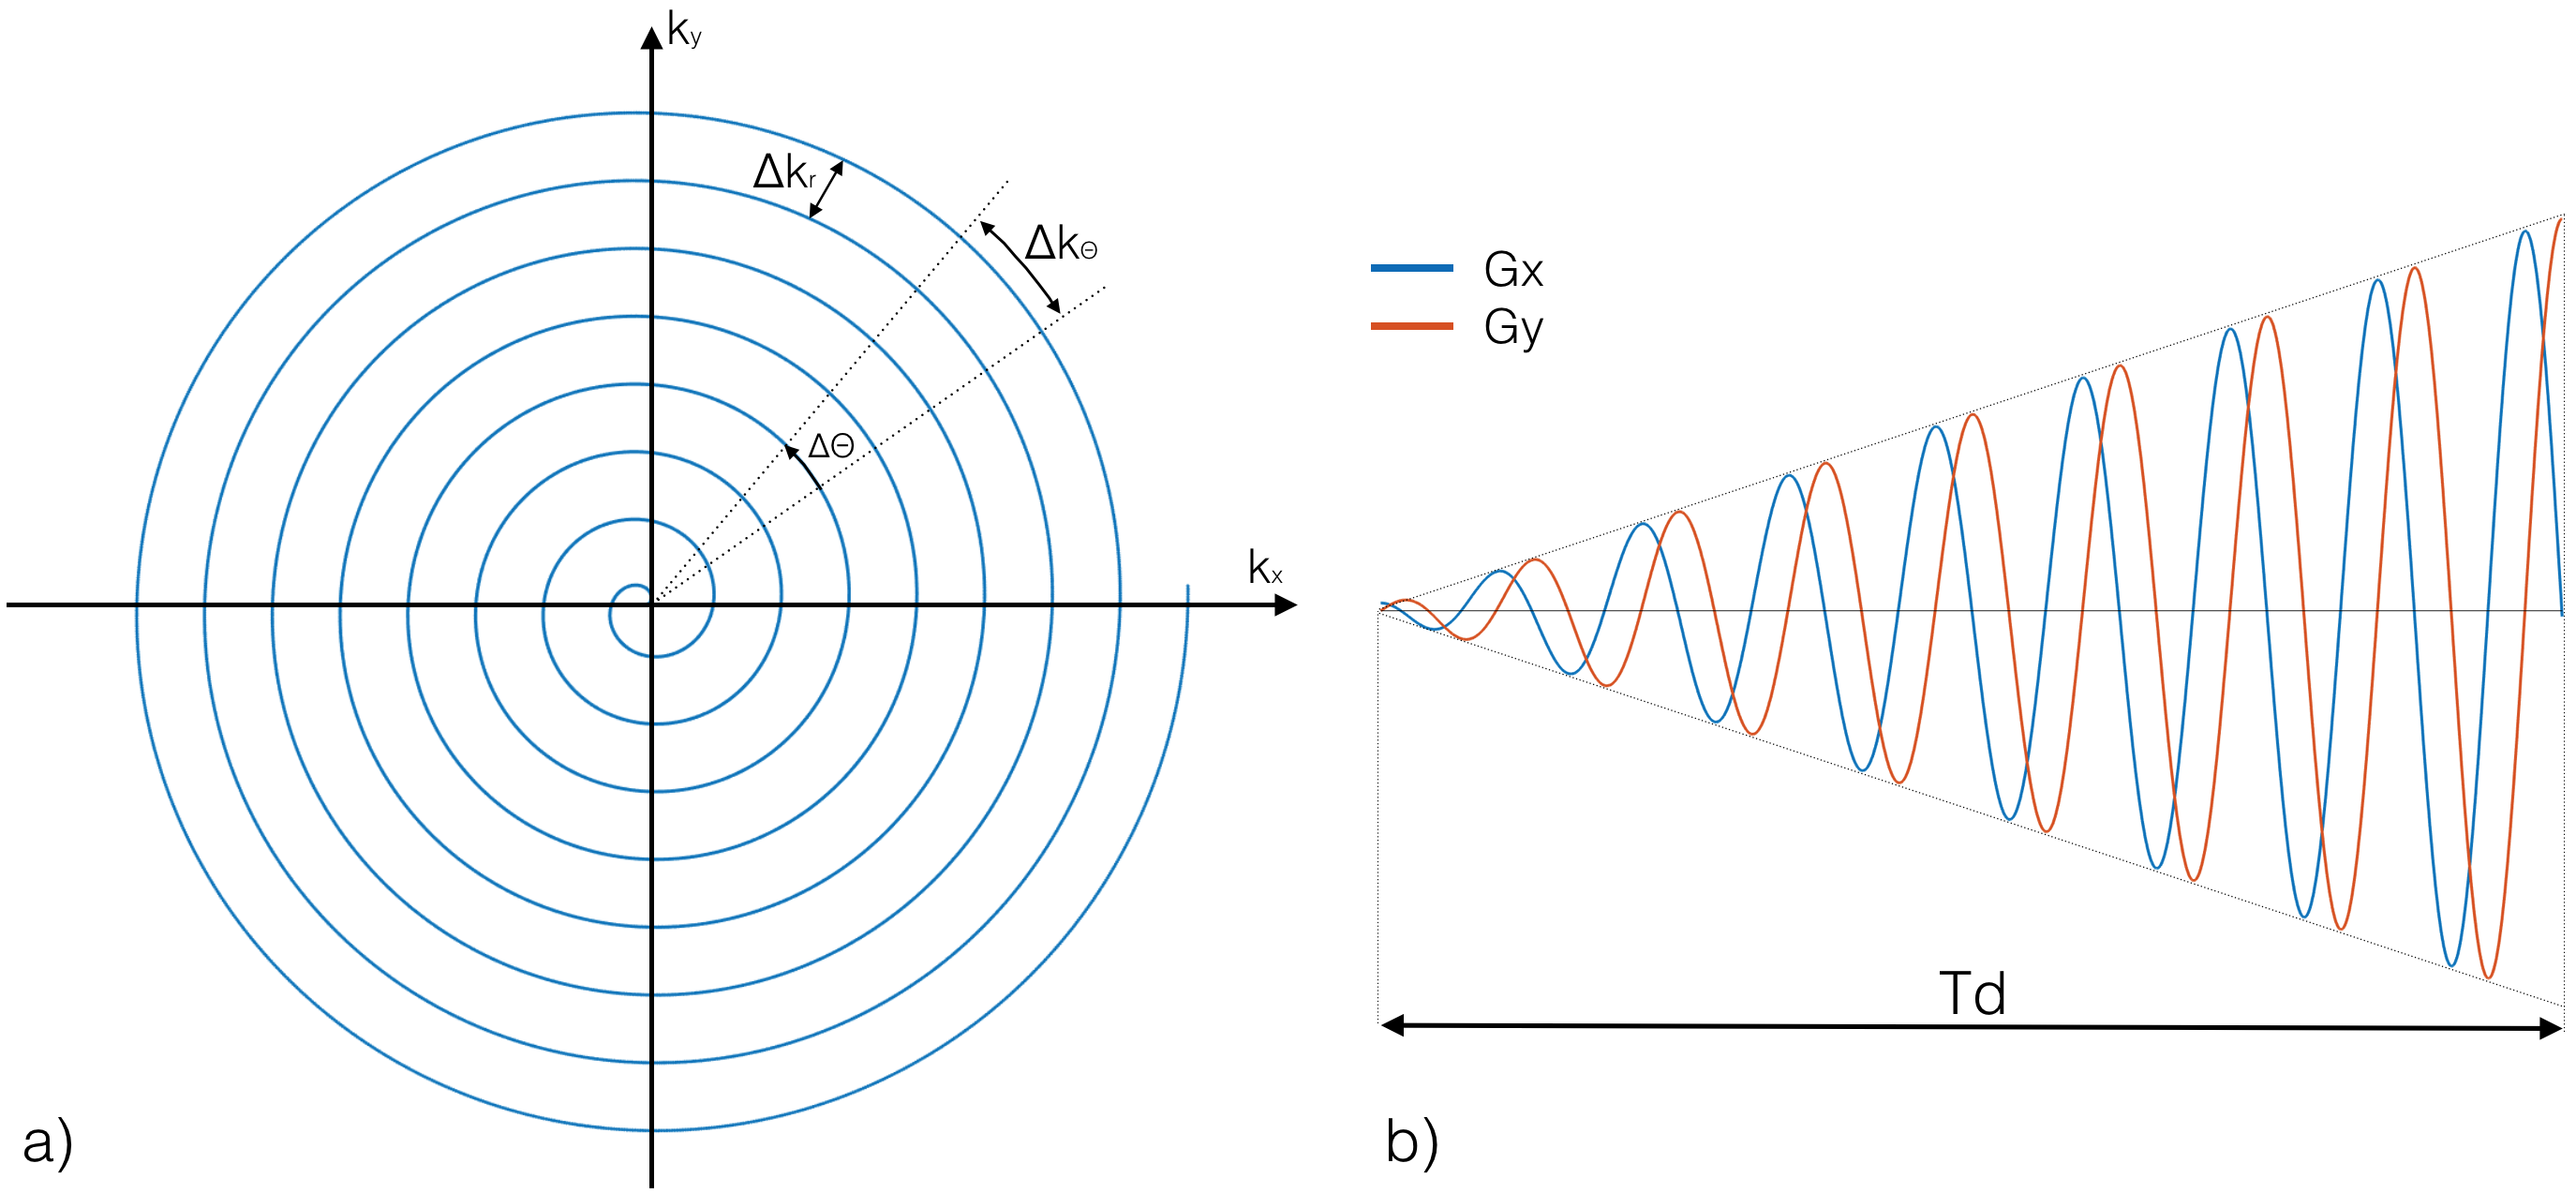
\includegraphics[angle=0,width=1\textwidth, keepaspectratio]{images/mrf/spiralAcquisition}
    \caption{An illustration of the linearly increasing spiral acquisition, showing a) the k-space trajectory and b) the corresponding gradient shape for this trajectory}
    \label{fig:spiralAcquisition}
\end{figure}

The spiral readout was constructed in JEMRIS by analytically describing the shape of the k-space trajectory.
While different spiral coverages of k-space exist, for our simulations we chose a linearly increasing sinusoidal form, also known as a constant angular velocity (Archimedean) spiral trajectory first proposed by Ahn et al. \cite{Ahn1986}. 
Mathematically, the k-space trajectory takes the following form:

\begin{equation}\label{eq:kspacespiral}
    \begin{split}
        k_x(t) &= \text{\sout{$\gamma$}} \, \, \alpha_1 t \, \, cos (\alpha_2 t) \\
        k_y(t) &= \text{\sout{$\gamma$}}  \, \, \alpha_1 t  \, \, sin (\alpha_2 t) 
    \end{split}
\end{equation}

where $\alpha_1$ determines the gradient amplitude and $\alpha_2$ determines the angular frequency.
From equation \ref{eq:kspacespiral} and from knowing that $k_x(t) = \text{\sout{$\gamma$}} \, \, \int_0^t G_x(t') dt'$ and $k_y(t) = \text{\sout{$\gamma$}} \, \, \int_0^t G_y(t') dt'$ (see equation \ref{eq:kspace}), the desired time domain gradients can be found:

\begin{equation}
    \begin{split}
        G_x(t) &= \frac{1}{\text{\sout{$\gamma$}}} \frac{d}{dt} \,\, [k_x(t)] = \alpha_1 cos (\alpha_2 t) - \alpha_1 \alpha_2 t sin (\alpha_2 t) \\
        G_y(t) &= \frac{1}{\text{\sout{$\gamma$}}} \frac{d}{dt} \,\, [k_y(t)] = \alpha_1 sin (\alpha_2 t) + \alpha_1 \alpha_2 t cos (\alpha_2 t) 
    \end{split}
\end{equation}

The shape of both the k-space trajectory and the gradient waveforms can be seen in Figure~\ref{fig:spiralAcquisition}, where $t \in [0, T_d]ms$.

\hfill

Constant angular velocity Archimedean spirals have constant step sizes in both radial ($\Delta k_r$) and azimuthal directions ($\Delta k_{\theta}$).
The values for these step sizes can be found by considering the sampling requirements imposed by the Nyquist criterion.
For this, we first need to rewrite the k-space trajectory in polar coordinates:
\begin{equation}
    \begin{split}
        k_r(t) &= \sqrt{k_x^2(t) + k_y^2(t)} = \text{\sout{$\gamma$}} \alpha_1 t \\
        k_{\theta}(t) &= tan^{-1} \Bigg[ \frac{k_y(t)}{k_x(t)} \Bigg] = \alpha_2 t
    \end{split}
\end{equation}

Now, considering constant numbers of sampling points per winding $n_{\theta}$ and radially $n_r$, and knowing that two radial points are exactly $2\pi$ apart, both angular and radial step sizes can be defined:
\begin{equation}\label{eq:deltak1}
    \Delta k_r = \text{\sout{$\gamma$}} \alpha_1 n_{\theta} \Delta t  \, \, \text{  and  } \, \, \Delta k_{\theta} = \alpha_2 \Delta t
\end{equation}
where $\Delta t$ is the sampling rate.
% \Delta k_r = k_r(t) \rvert_{t=t'+2\pi/\alpha_2} + k_r(t) \rvert_{t=t'}
To find the required number of sampling points, we can also write:
\begin{equation}\label{eq:deltak2}
    \Delta k_r = \frac{k_{max}}{n_r} = \frac{1}{2 \Delta r n_r} \leq \frac{1}{L} \, \, \text{  and  } \, \,  \Delta k_{\theta} = k_{max} \Delta \theta = \frac{2 \pi}{2 \Delta r n_{\theta}} \leq \frac{1}{L} 
\end{equation}
where $\Delta r$ is the image resolution.
Therefore, for a fully sampled spiral we choose: $n_r \geq L / 2 \Delta r$ and $n_{\theta} \geq \pi L / \Delta r$.

\hfill

Explicit values for $\alpha_1$ and $\alpha_2$ are found from equations \ref{eq:deltak1} and \ref{eq:deltak2}:
\begin{equation}
    \alpha_1 = \frac{\pi}{\text{\sout{$\gamma$}} n_{\theta} n_r \Delta t \Delta r}  \, \, \text{  and  } \, \, \alpha_2 = \frac{2 \pi}{n_{\theta} \Delta t}
\end{equation}
%The total required acquisition time will therefore be: $T_d = n_r n_{\theta} \Delta t$.
and
\begin{equation}
    \Delta t = \frac{T_d}{n_r n_{\theta}}
\end{equation}

\hfill

To reconstruct our input object in a matrix size of $128 \times 128$ with an image resolution of $\Delta r = 1.25mm$,
%circular field-of-view of $160mm$ diameter encompassing our object.
%This means that our image resolution was $\Delta r = 1.25mm$.
%Therefore, we required $n_r \geq \frac{L}{2 \Delta r} = 64$ and
we required $n_r \geq \frac{L}{2 \Delta r} = 64$ and
$n_{\theta} \geq \frac{\pi L}{\Delta r} = 403$.
This means we had to sample approximately $25,792$ times every readout.
For a total acquisition time of $T_d = 6ms$, we calculated a dwell time of $\Delta t = 0.233 \mu s$.
The slice thickness was set to $1mm$, but as we used a 2D input object, there were no slice selection gradients introduced in the simulations.

% Now, considering a constant number of sampling points per winding $n_{\theta}$ and an angular step size $\Delta \theta$, the complete angular coverage of one full turn of the spiral is defined by:
% \begin{equation}
%     2\pi = n_{\theta} \Delta \theta
% \end{equation}
% Moreover, since an angle $\Delta \theta$ is covered at each sampling interval $\Delta t$, the angular frequency $\alpha_2$ becomes:
% \begin{equation}
%     \alpha_2 \equiv \frac{\Delta \theta}{\Delta t} = \frac{2\pi}{n_{\theta}\Delta t}
% \end{equation}
% 
% This value can be found through a simple trigonometric argument.
% By defining $\Delta \theta$ as the step size in the azimuthal direction
% 
% In order to do so, we first need to adapt the step sizes in k-space to polar coordinates.
% the k-space trajectory in polar coordinates:

\hfill

% % % % % % % % % % % % 
\subsubsection{Reconstruction}

Spiral k-space coverage leads to a non-Cartesian distribution of sampled points in k-space.
In order to reconstruct the image, a simple 2D-FFT will not suffice.
The alternative, described in more detail in Appendix~\ref{MRIgridding}, is called `gridding'.
In our work we used the inverse gridding function provided by the BART toolbox \cite{Lustig2016}.
The Berkeley Advanced Reconstruction Toolbox (BART) is an open-source framework that provides command-line tools for many image-reconstruction algorithms commonly used in Magnetic Resonance Imaging.

\hfill

BART's \texttt{nufft} command line tool requires two types of inputs to reconstruct an image: the k-space trajectory and the signal samples.
Both sets of values were collected as a result of the JEMRIS simulations and then fed to BART.
As a result, a set of $N = 500$ images was obtained, where $N$ is the number of repetition blocks.

\hfill

% % % % % % % % % % % % 
\subsubsection{Motion}
\label{method:motion}

In-plane motion was introduced in three sets of experiments by corrupting $1.5$ seconds worth of scan time out of a total of $7.5$ seconds.
The chosen three motion types are:
\begin{enumerate}
    \item \textit{Motion 1}: Continuous rotation about the z-axis ($10^o$ rotation)
    \item \textit{Motion 2}: Continuous translation along the y-axis ($10mm$ translation)
    \item \textit{Motion 3}: Both rotation about the z-axis and translation along the y-axis ($10^o$ rotation and $10mm$ translation)
\end{enumerate}

All three types of motion had varying times of onset: at the beginning of the scan, in the middle of the scan, and at the end of the scan.

% \hfill

% The four steps described above are summarised in Figure~\ref{fig:pipeline}.

% \begin{figure}[ht]
%     \centering
%     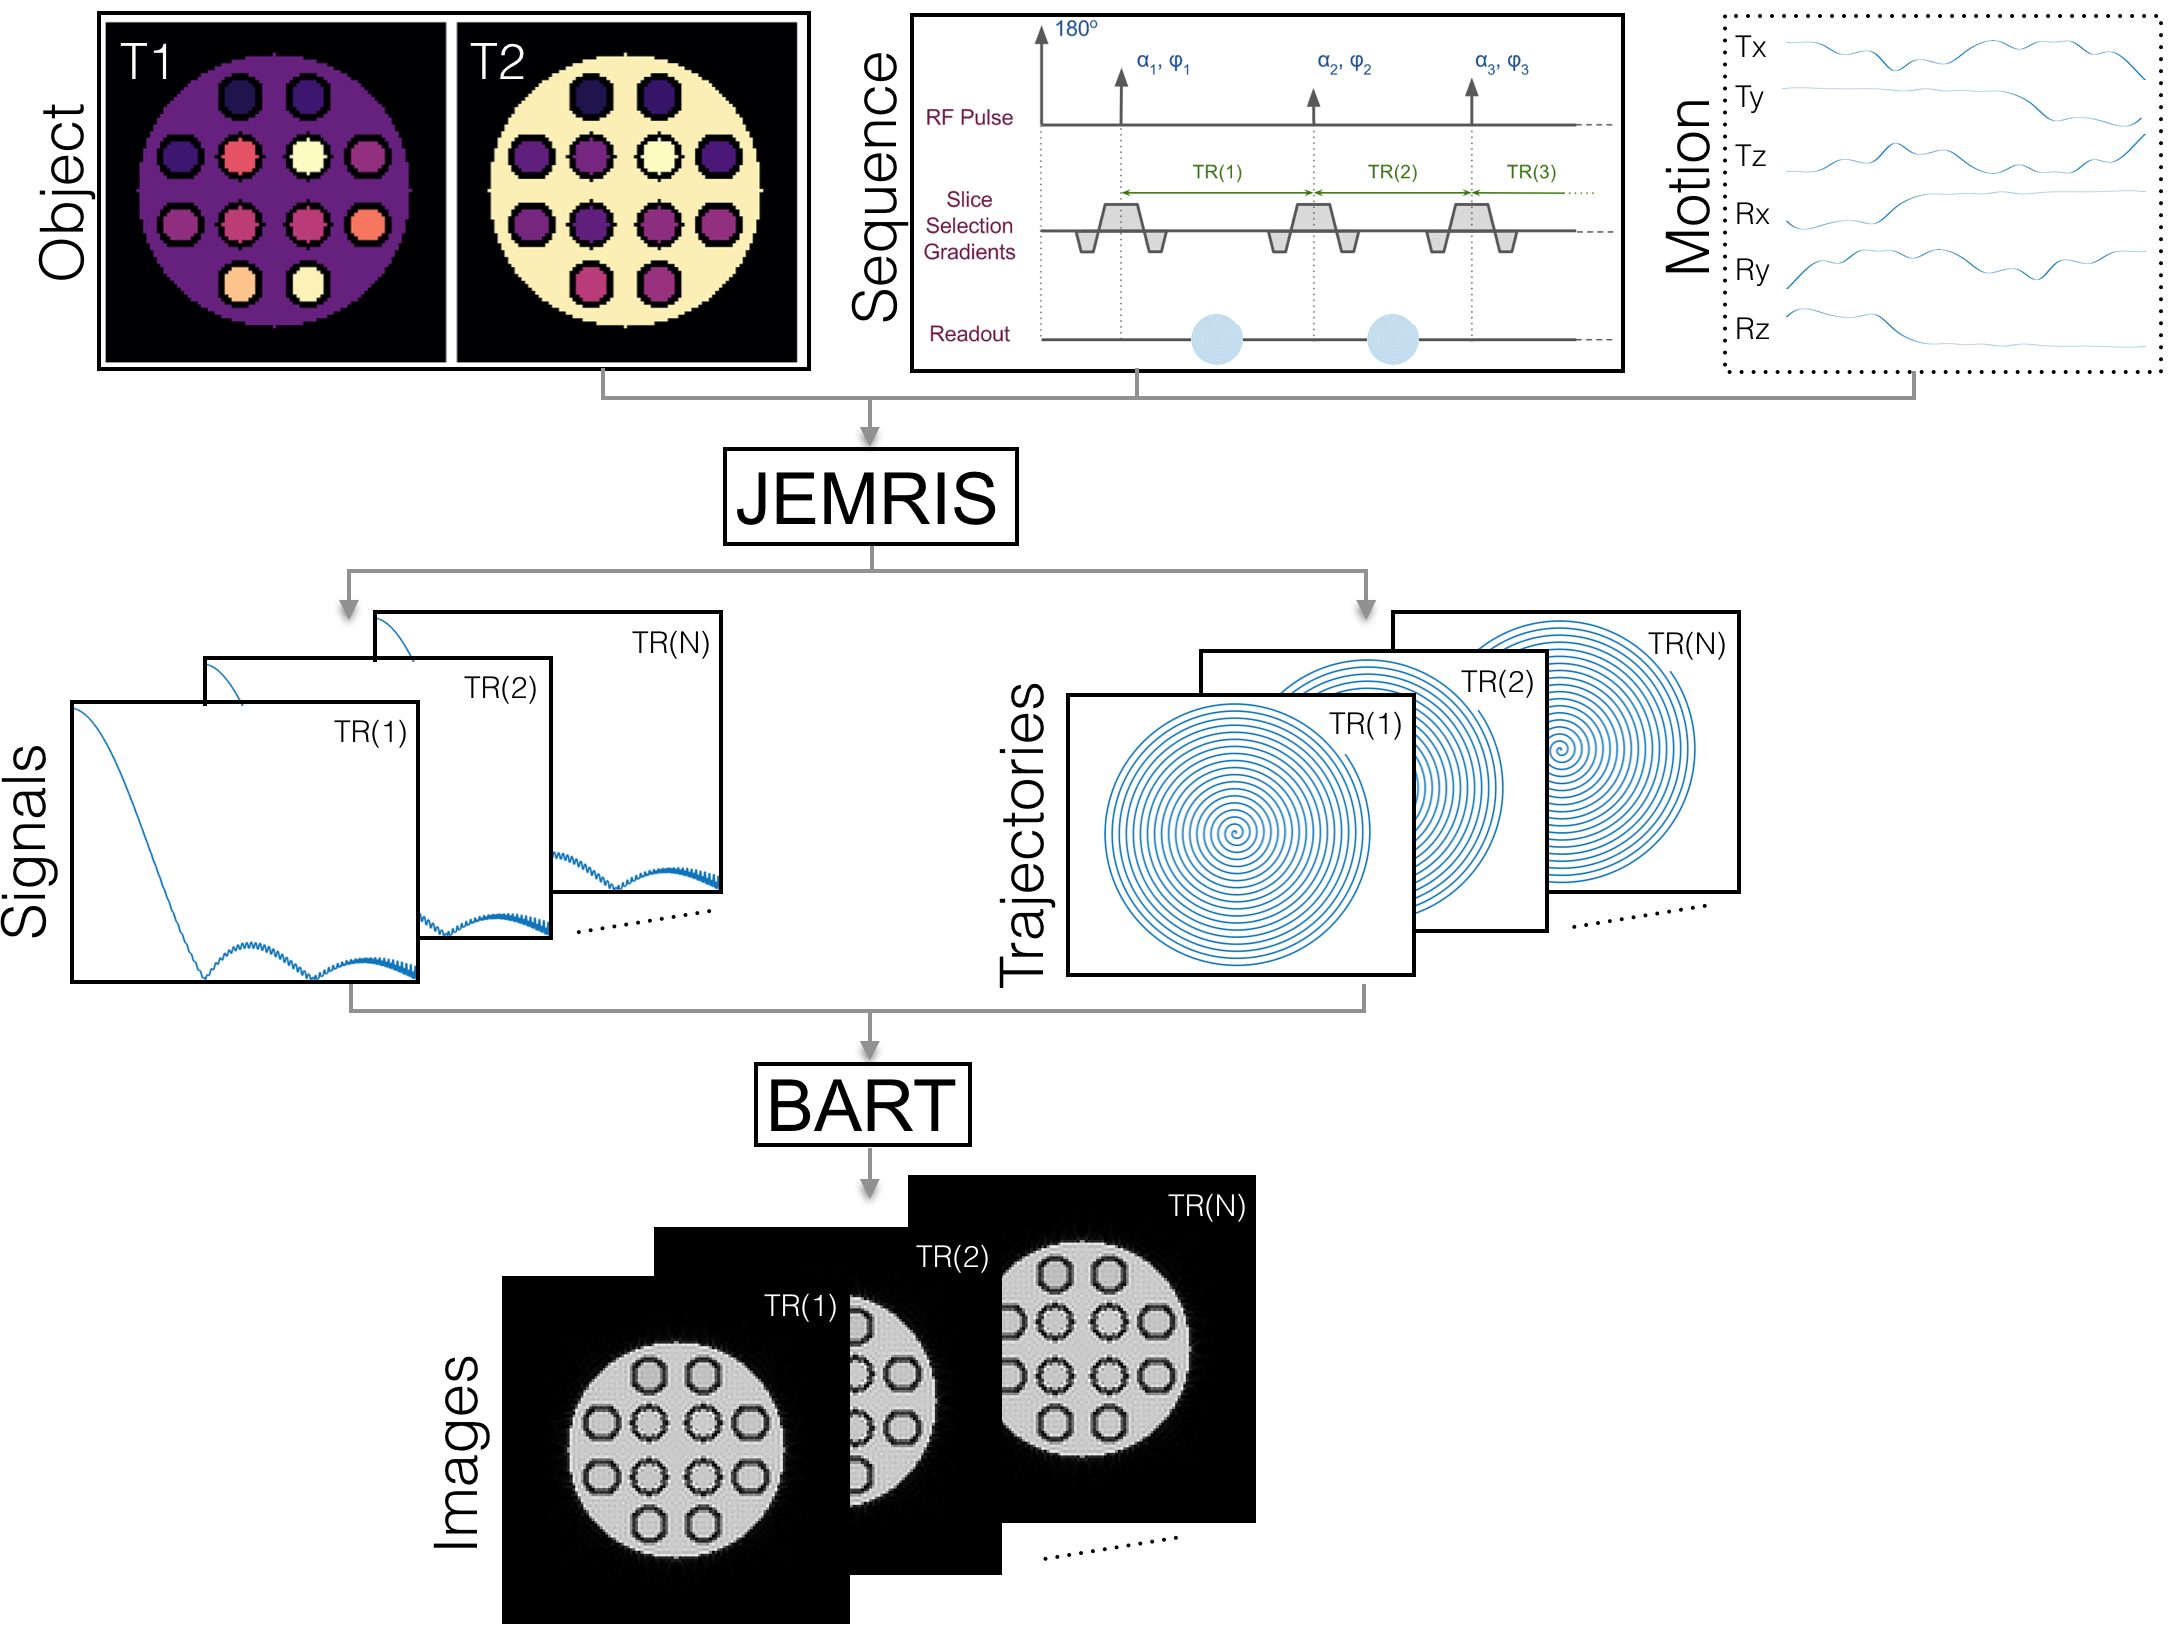
\includegraphics[angle=0,width=1\textwidth, keepaspectratio]{images/mrf/pipelineWithMotion}
%     \caption{Summary of the pipeline used to simulate the images}
%     \label{fig:pipeline}
% \end{figure}

\hfill

% % % % % % % % % % % % % % % % % % % % % % % % % % % % % % % % % % % % % % % % % % % % % % % % % % % % % % % % % % % % % % % % % % % % % % % % % % % % % % % % % % % % % % % % % % % % % % % % % % % % % % % % % % % % % % % % % % % % % % % % % % % % % % % % % % % % % % % % % % % % % % % % 
\subsection{Matching Algorithm}
\label{method:matching}

The pattern matching algorithm used is the same as described in the original MRF implementation \cite{Ma2013}.
It involves a vector dot-product between all the simulated image-space signals and the precomputed dictionary, and the retrieval of the dictionary signal which gives the highest score.
Prior to computing the dot-product, both types of signals are normalised to each having the same sum squared magnitude.
%Conceptually, the two signals need to be as `similar' as possible to say that a certain pair of tissue properties can be attributed to the observed signal.

\hfill

Mathematically, this can be described with the following formulation.
Let there be a dictionary $D \in \mathfrak{C}^{M \times N}$, where M is the number of parameter combinations and N is the number of timepoints.
Any dictionary signal $d_j$, with $j \in [1,M]$, represents the $j^{th}$ row of $D$.
Then, the process of pattern matching involves finding the dictionary entry $d_l$ which satisfies:
\begin{equation}
    d_l = \arg\!\max_{d_j} \, \lvert d_j \, x^* \rvert
\end{equation}
where $x$ is the image-space signal and $x^*$ is the conjugate transpose of $x$.
Both the dictionary entry and the image space signal have to be normalised to have unit length: $\lvert \lvert x \rvert \rvert = \lvert \lvert d_j \rvert \rvert = 1$, where $\lvert \lvert \, \cdot \, \rvert \rvert$ is the Euclidean norm.
Once the match is recovered, the voxel corresponding to the image space signal $x$ is assigned the tissue parameters used to generate the matching entry's signal.

\hfill

This process is then repeated for all the image space signals corresponding to all the voxels in the image dataset.
At the end, a set of tissue parameter maps is created.